\documentclass[aspectratio=169,10pt]{beamer}
\usepackage[T1]{fontenc}
\usepackage[utf8]{inputenc}
\usepackage[english]{babel}
\usepackage{lmodern}
\usepackage{amsmath,amssymb,booktabs,graphicx}
\usetheme{Madrid}
\definecolor{navy}{RGB}{22,50,79}
\definecolor{teal}{RGB}{8,126,139}
\setbeamercolor{structure}{fg=navy}
\setbeamercolor{frametitle}{bg=navy,fg=white}
\setbeamercolor{block title}{bg=teal,fg=white}
\setbeamertemplate{navigation symbols}{}
\setbeamertemplate{footline}[frame number]
\setbeamertemplate{itemize items}[circle]
\graphicspath{{assets/}}
\setbeameroption{hide notes}
\title{MNIST MLP from Scratch}
\subtitle{Learning neural network foundations with Python and NumPy}
\author{MLP-from-Scratch contributors}
\date{15 November 2026}
\begin{document}
\begin{frame}\titlepage\end{frame}
\section{Part 1: Neural Network Fundamentals}
\begin{frame}{Part 1: Neural Network Fundamentals}
\tableofcontents[currentsection]\end{frame}

\begin{frame}{Why we implemented an MLP}
\begin{itemize}
\item We wanted to connect matrix operations and derivatives to a working learning system.
\item We implemented every learning operation in Python and NumPy.
\item Our goal is a reproducible educational baseline, not a state-of-the-art claim.
\end{itemize}
\end{frame}

\begin{frame}{What is a neural network?}
\[f_{\theta}(x)=W_L^{\top}\,\phi(\cdots\phi(W_1^{\top}x+b_1)\cdots)+b_L\]\begin{itemize}
\item A parameterized function that maps inputs to outputs.
\item Layers combine evidence; nonlinear activations make the composition expressive.
\item In supervised learning, labeled examples guide parameter updates.
\end{itemize}

\note{The expression illustrates a column-vector convention; our implementation stores batches in rows.}
\end{frame}

\begin{frame}{Biological and artificial neurons}
\begin{tabular}{p{.43\textwidth}p{.48\textwidth}}\toprule Biological neuron & Artificial neuron\\\midrule Dendrites receive signals & Inputs contain numerical features\\[6pt] Synapses influence transmission & Weights scale each input\\[6pt] Cell dynamics produce electrical activity & An activation transforms a weighted sum\\\bottomrule\end{tabular}\vspace{10pt}This is an intuition, not a faithful simulation of a brain.\end{frame}

\begin{frame}{Weights and biases}
\[z=\sum_{j=1}^{d}w_jx_j+b,\qquad a=\phi(z)\]\begin{itemize}
\item A weight controls the contribution of an input; its sign can support or oppose a response.
\item The bias shifts the response even when inputs are zero.
\item We learn weights and biases; we choose learning rate and architecture as hyperparameters.
\end{itemize}
\[x=(0.2,0.8),\quad w=(0.5,-0.25),\quad b=0.2\quad\Rightarrow\quad z=0.1\]\end{frame}

\begin{frame}{ReLU activation}
\[\operatorname{ReLU}(z)=\max(0,z),\qquad \operatorname{ReLU}^{\prime}(z)=\mathbf{1}_{z>0}\]\begin{itemize}
\item Positive values pass through; negative values become zero.
\item Without nonlinear activations, stacked affine layers reduce to one affine map.
\item We choose derivative zero at zero and use He initialization for hidden layers.
\end{itemize}
\[W_{ij}\sim\mathcal{N}(0,2/n_{\mathrm{in}}),\qquad b=0\]\end{frame}

\begin{frame}{Our architecture}
\[784\;\longrightarrow\;128\;\longrightarrow\;64\;\longrightarrow\;10\]\begin{itemize}
\item Two dense hidden layers with ReLU; a linear output layer returns ten logits.
\item 109,386 trainable parameters, including biases.
\item The output weights use Xavier initialization; hidden weights use He.
\end{itemize}
\[(784\cdot128+128)+(128\cdot64+64)+(64\cdot10+10)=109386\]\end{frame}

\begin{frame}{Forward pass for a batch}
\[Z^{(\ell)}=A^{(\ell-1)}W^{(\ell)}+b^{(\ell)}\]\[X\in\mathbb{R}^{B\times784}\to A^{(1)}\in\mathbb{R}^{B\times128}\to A^{(2)}\in\mathbb{R}^{B\times64}\to Z^{(3)}\in\mathbb{R}^{B\times10}\]\begin{itemize}
\item Each row is one image; matrix multiplication processes the batch together.
\item Training caches inputs and ReLU masks for backward propagation.
\end{itemize}
\end{frame}

\begin{frame}{Softmax and the predicted class}
\[p_{ic}=\frac{\exp(z_{ic}-m_i)}{\sum_k\exp(z_{ik}-m_i)},\qquad m_i=\max_k z_{ik}\]\[\widehat y_i=\operatorname*{arg\,max}_{c}p_{ic}\]\begin{itemize}
\item Subtracting the maximum preserves probabilities and avoids exponential overflow.
\item Scores sum to one; high scores do not guarantee correctness or calibration.
\end{itemize}
\end{frame}

\section{Part 2: Dataset Overview}
\begin{frame}{Part 2: Dataset Overview}
\tableofcontents[currentsection]\end{frame}

\begin{frame}{MNIST handwritten digits}
\centering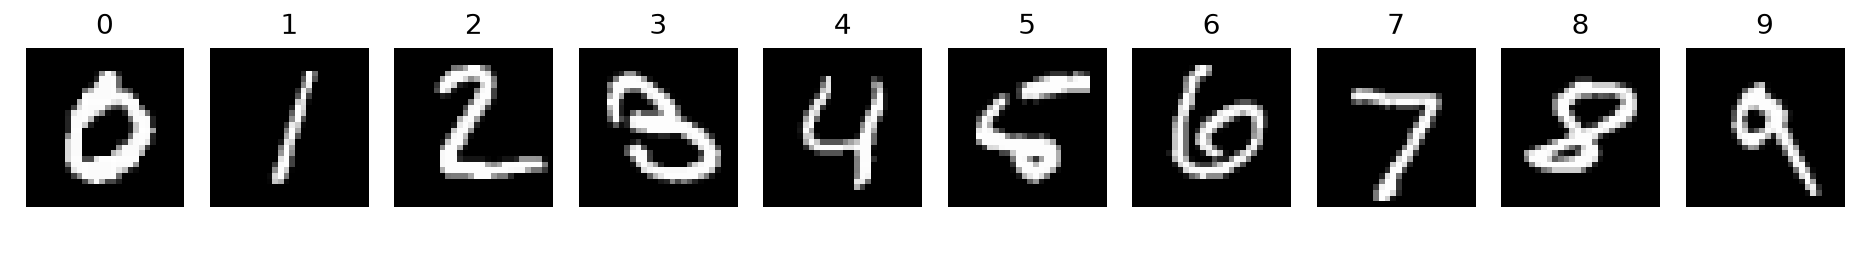
\includegraphics[width=\textwidth]{mnist.png}\par\raggedright\begin{itemize}
\item Ten classes: digits 0 through 9, with grayscale images and known labels.
\item The original partitions contain 60,000 training and 10,000 test images.
\item We verify downloaded archives and decode the IDX format ourselves.
\end{itemize}
\scriptsize Dataset: LeCun, Cortes and Burges. Images are actual test examples.\end{frame}

\begin{frame}{Flattening and normalization}
\[28\times28=784,\qquad x_j=\frac{\mathrm{pixel}_j}{255}\in[0,1]\]\begin{itemize}
\item We convert pixels to float32 and read rows in a fixed order.
\item Inputs have shape (N, 784); integer labels have shape (N,).
\item The MLP sees values at fixed positions, without a built-in spatial neighborhood operation.
\end{itemize}
\end{frame}

\begin{frame}{Training, validation and test}
\begin{center}\begin{tabular}{lrl}\toprule Partition & Images & Purpose\\\midrule Training & 50,000 & Update weights\\ Validation & 10,000 & Select settings and checkpoint\\ Official test & 10,000 & Evaluate after selection\\\bottomrule\end{tabular}\end{center}\begin{itemize}
\item We split only the original training pool, using stratification and seed 42.
\item We use normalization only: no deskewing or augmentation in this run.
\end{itemize}
\end{frame}

\section{Part 3: Learning Process and Results}
\begin{frame}{Part 3: Learning Process and Results}
\tableofcontents[currentsection]\end{frame}

\begin{frame}{Cross-entropy loss}
\[L=-\frac1B\sum_{i=1}^{B}\sum_{c=0}^{9}Y_{ic}\log p_{ic}\]\begin{itemize}
\item Y is a one-hot representation of the correct classes; the loader keeps integer labels.
\item A low score for the correct class receives a larger penalty.
\item We compute the loss directly from logits using shifted log-sum-exp.
\end{itemize}
\[L_i=\log\sum_k e^{z_{ik}-m_i}-(z_{i,y_i}-m_i)\]\end{frame}

\begin{frame}{Backpropagation and the chain rule}
\[\frac{\partial L}{\partial w}=\frac{\partial L}{\partial z}\,\frac{\partial z}{\partial w}\]\[\frac{\partial L}{\partial Z^{(3)}}=\frac{P-Y}{B}\]\begin{itemize}
\item We move gradients backward through the composition of layers.
\item The gradient measures local sensitivity, not an independent error for each neuron.
\item The batch average is applied once, in the loss gradient.
\end{itemize}
\end{frame}

\begin{frame}{Gradients of a dense layer}
\[dW=A_{\mathrm{previous}}^{\top}dZ,\qquad db=\sum_{i=1}^{B}dZ_i\]\[dA_{\mathrm{previous}}=dZ\,W^{\top},\qquad dZ_{\mathrm{ReLU}}=dA\odot\mathbf1_{Z>0}\]\begin{itemize}
\item Gradient shapes match their parameters; bias gradients retain shape (1, n-out).
\item We compute all gradients before updating any weights.
\end{itemize}
\end{frame}

\begin{frame}{Mini-batch SGD}
\[\theta_{t+1}=\theta_t-\eta\nabla_{\theta}L_{\mathrm{batch}}\]\begin{itemize}
\item We use learning rate 0.1 and batch size 64, including the final partial batch.
\item We shuffle the training order every epoch.
\item An epoch is one complete pass over the training examples.
\item We run 20 epochs; seed 42 controls initialization, splitting and shuffling.
\end{itemize}
\end{frame}

\begin{frame}{Our training workflow}
\begin{itemize}
\item For each batch: forward, loss, backward, SGD update.
\item At epoch end: recompute sample-weighted training and validation metrics.
\item We save the checkpoint with minimum validation loss.
\item We freeze selection before measuring official test performance.
\end{itemize}
\small\texttt{data/mnist.py} $\to$ \texttt{network.py} $\to$ \texttt{trainer.py} $\to$ \texttt{evaluate.py}\end{frame}

\begin{frame}{Loss and accuracy during training}
\centering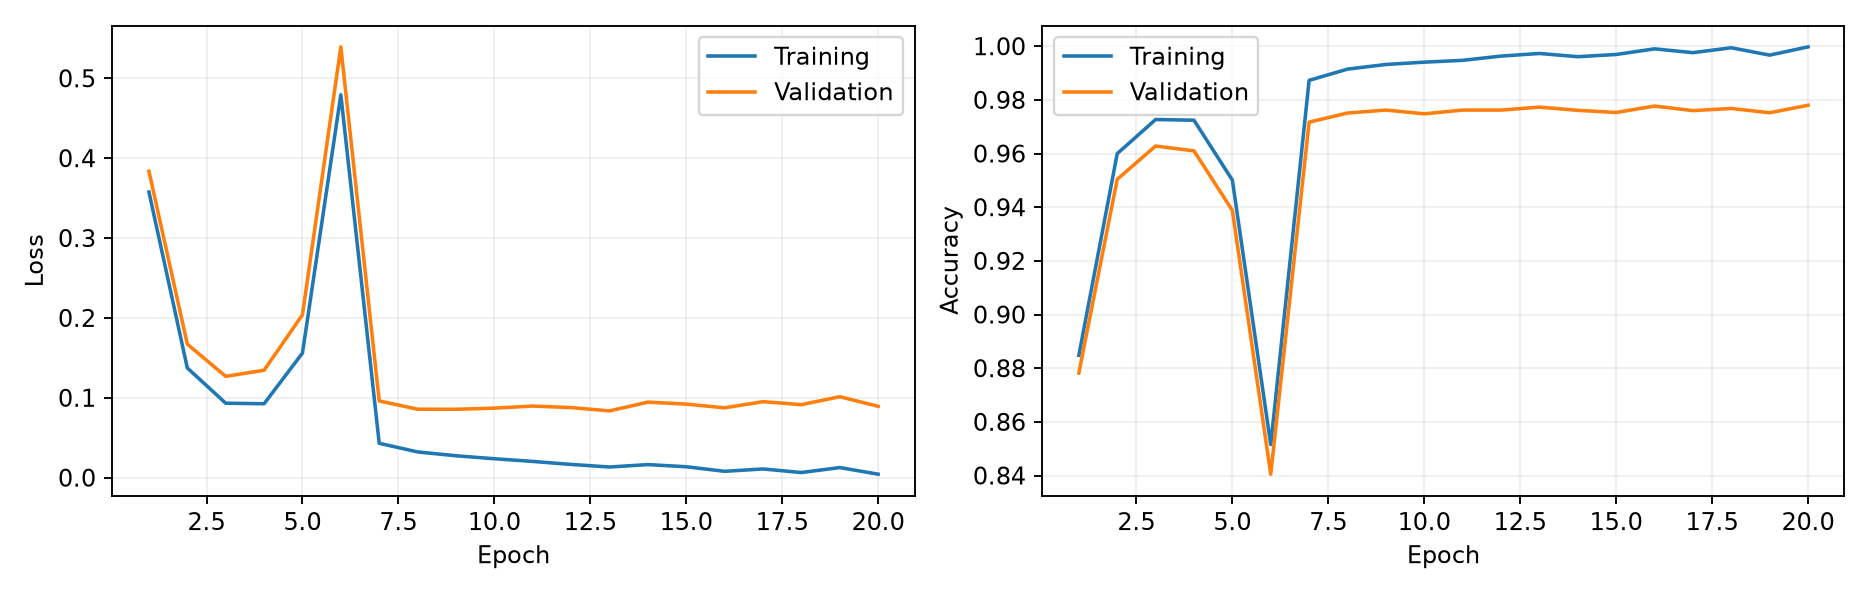
\includegraphics[width=.94\textwidth]{curves_en.png}\par\raggedright\begin{itemize}
\item Validation loss was lowest at epoch 13: 0.083610; accuracy was 97.73\%.
\item Later training improvements did not consistently improve validation loss.
\end{itemize}
\end{frame}

\begin{frame}{Final evaluation of the selected checkpoint}
\begin{center}\begin{tabular}{lr}\toprule Test metric & Measured result\\\midrule Accuracy & 97.90\%\\ Correct / incorrect & 9,790 / 210\\ Cross-entropy & 0.072777\\ Macro precision / recall & 97.90\% / 97.87\%\\ Macro / weighted F1 & 97.88\% / 97.90\%\\ Macro / micro ROC AUC & 0.999621 / 0.999617\\\bottomrule\end{tabular}\end{center}One run, one seed, 10,000 official test images.\par\scriptsize\texttt{results/baseline/extended\_metrics.json}\end{frame}

\begin{frame}{Confusion matrix}
\begin{columns}[c]\column{.53\textwidth}\centering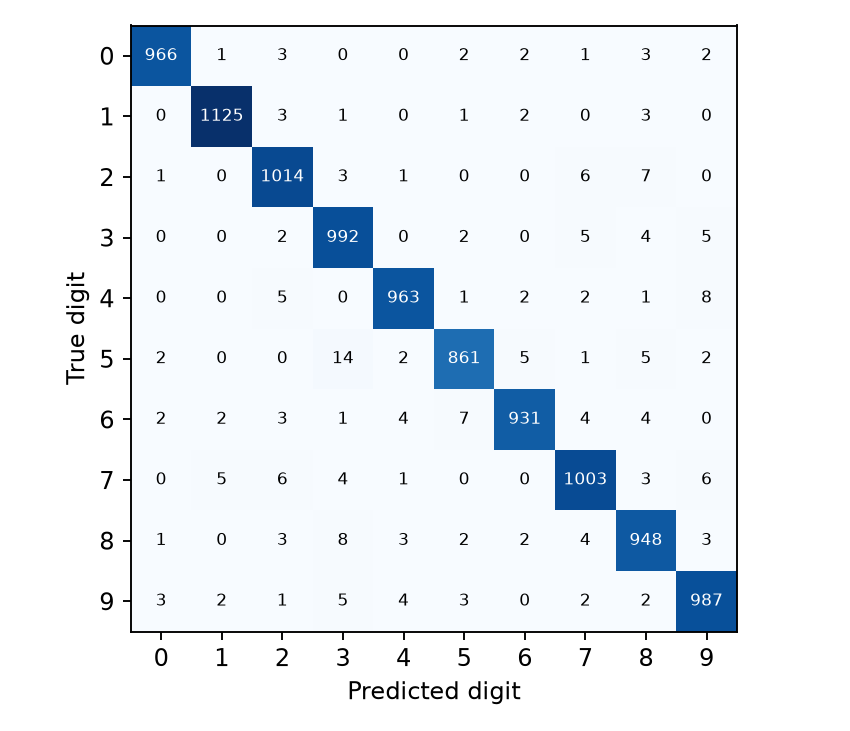
\includegraphics[width=\linewidth,height=.65\textheight,keepaspectratio]{confusion_en.png}\column{.45\textwidth}\begin{itemize}
\item Rows are true digits; columns are predicted digits.
\item The largest directed error: 5 predicted as 3, with 14 cases.
\item Digit 8 had the lowest F1: 97.03\%.
\end{itemize}
\end{columns}\end{frame}

\begin{frame}{ROC curves and one-vs-rest AUC}
\begin{columns}[c]\column{.53\textwidth}\centering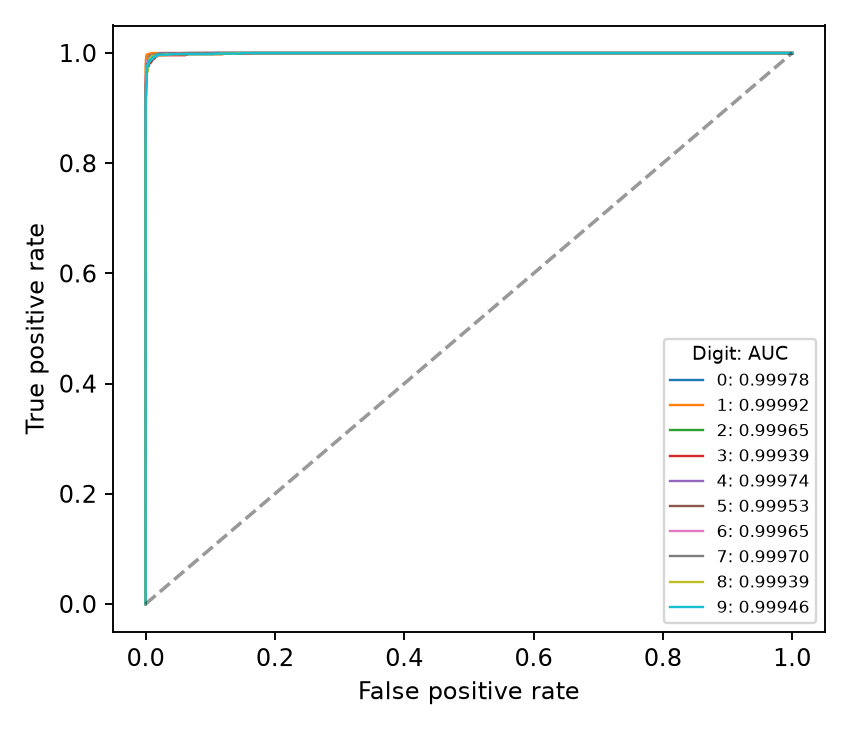
\includegraphics[width=\linewidth,height=.65\textheight,keepaspectratio]{roc_en.png}\column{.45\textwidth}\begin{itemize}
\item For each digit, vary a threshold on its score against all other digits.
\item Macro averages ten AUCs; micro pools image/class pairs.
\item High ranking AUC is not the same as multiclass accuracy or calibration.
\end{itemize}
\end{columns}\end{frame}

\begin{frame}{Real mistakes and confident wrong answers}
\centering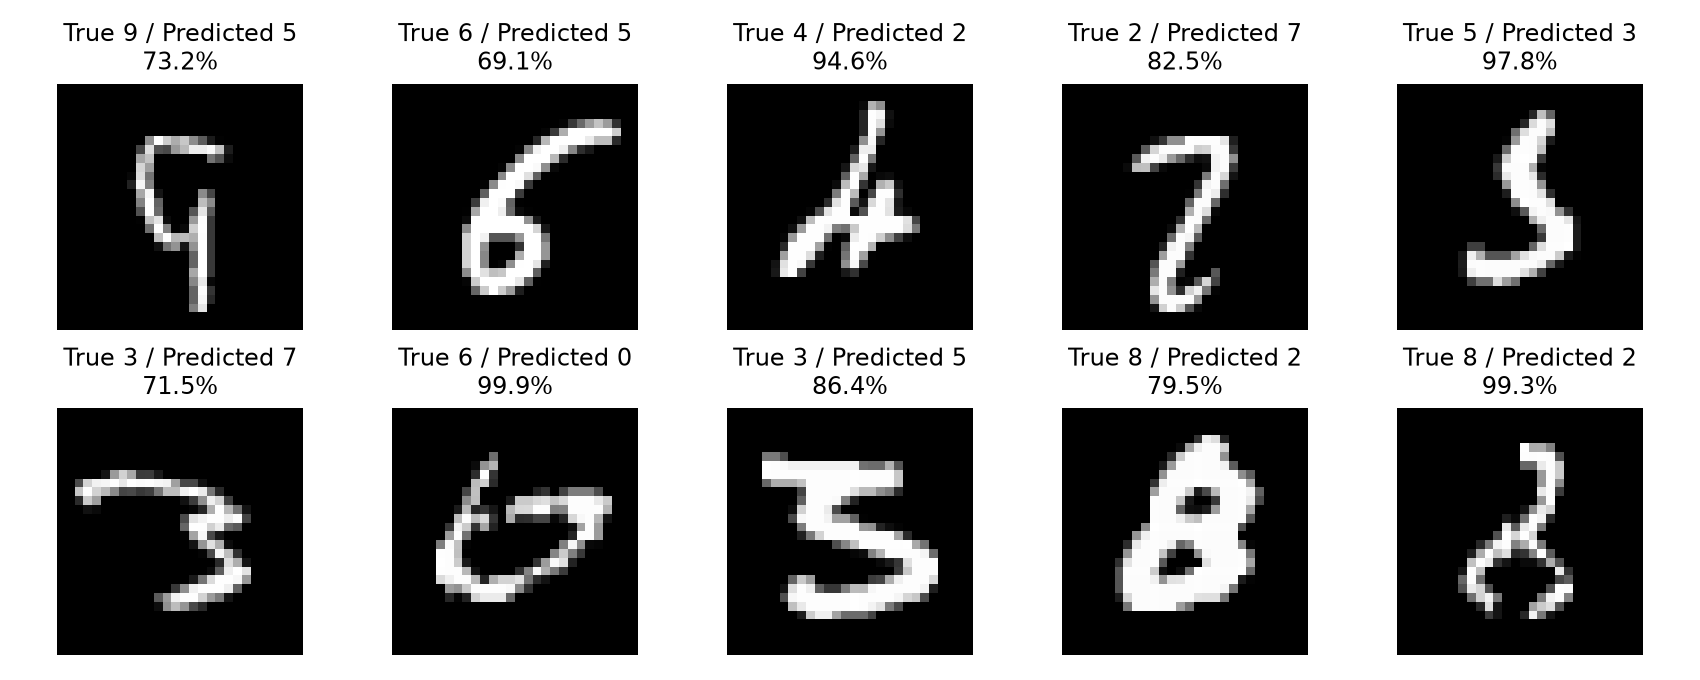
\includegraphics[width=.92\textwidth,height=.61\textheight,keepaspectratio]{errors_en.png}\par\raggedrightFirst ten mistakes in test order, not a hand-picked selection. Values are the predicted-class Softmax scores.\end{frame}

\begin{frame}{Verification and limitations}
\begin{itemize}
\item 24 tests cover finite-difference gradients, stable loss, tied ROC scores, serialization and training.
\item The fixed-model Wilson 95\% accuracy interval is 97.60--98.16\%, under a binomial assumption.
\item One seed does not establish variation across runs; Softmax outputs are not calibrated.
\item We would compare seeds, learning-rate schedules and regularization on validation data.
\end{itemize}
\end{frame}

\begin{frame}{What we learned and where to look}
\begin{itemize}
\item We connected data preparation, forward propagation, gradients and optimization.
\item Our result is reproducible evidence for this run, not a universal performance guarantee.
\item After inspecting test errors, future test-guided changes need fresh held-out evidence.
\end{itemize}
\small\url{https://github.com/jp-tedesco/MLP-from-Scratch}\par\texttt{docs/experiments.md}\quad\texttt{results/baseline/}\par\medskipDataset reference: LeCun, Cortes and Burges; CVDF MNIST mirror. All plots use our recorded checkpoint.\end{frame}

\end{document}
